\documentclass[a4j,11pt]{article}

\usepackage{amsmath,amssymb}
\usepackage{amsthm}


\usepackage{fontspec} %\set~font でフォント設定するにしろ必要
\usepackage{jpnreturn} % 作成したパッケージを読み込む

\setmainfont[ItalicFont=Times Italic]{Hiragino Mincho Pro} %セリフ(ローマン体)のフォント
\setsansfont[ItalicFont=Times Italic]{HiraKakuPro-W3} %サンセリフのフォント ItalicFont でイタリック設定
\setmonofont{HiraKakuPro-W3} %総称ファミリの \ttfamily(等幅,タイプライタ)に割り当てるファミリを指定する

%tikz
\usepackage{graphicx}
\usepackage{tikz}
\usetikzlibrary{automata,arrows}


\usepackage{wrapfig}
\usepackage{hyperref}


\DeclareMathOperator*{\argmin}{arg\,min}

\title{Oritatami Systemによる\\無限バイナリカウンタの実装}
\author{丸山晃平
\thanks{情報・ネットワーク工学専攻 1831144 関 研究室}
}
\date{令和 2年 1月 20日}%日付


\begin{document}
\maketitle

\section{はじめに}

\section{oritatami system とは}

\begin{equation}\label{eq:OS_CF}
C_{i+1} \in \argmin_{
\substack{
C \in \mathcal{C}_{\le \alpha} s.t. \\
C_i \xrightarrow{R}_{w[i+1]}C \\
}
}
\min \Bigl\{ \Delta G(C') \Bigm|
C \xrightarrow{R}^*_{w[i+2...i+k]}C', k\le \delta, C' \in \mathcal{C}_{\le \alpha}
\Bigr\}.
\end{equation}

「周囲の環境」の説明

\section{無限バイナリカウンタの実装}
この章では、oritatami system に実装した無限バイナリカウンタについて説明する。
ここで言う無限バイナリカウンタとは、あるビット幅でカウントアップしていたカウンタが桁上がりのためにオーバーフローした際に、そのビット幅を拡張することでカウントアップを無限に続けていくようなバイナリカウントを指す。

\begin{figure}[tb]
  \centering
   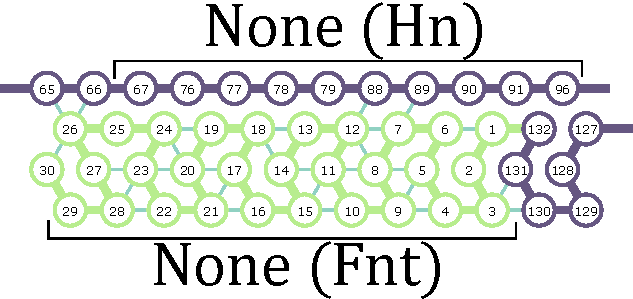
\includegraphics[width=0.6\linewidth]{fig/svg/Fnt_1.pdf}\\
 \vspace*{10mm}
   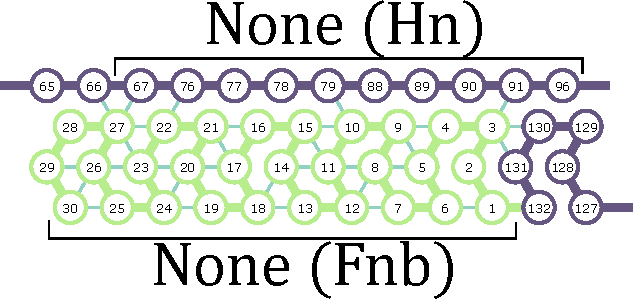
\includegraphics[width=0.6\linewidth]{fig/svg/Fnb_1.pdf}\\
 \vspace*{10mm}
   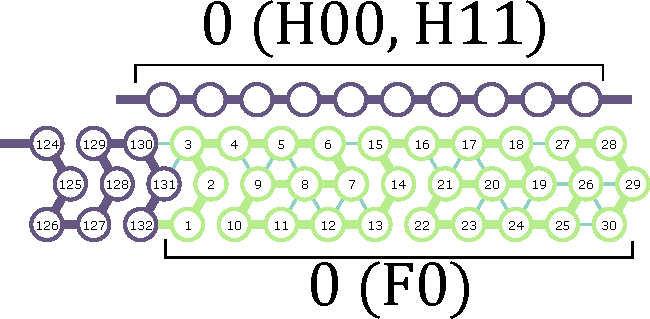
\includegraphics[width=0.6\linewidth]{fig/svg/F0_1.pdf}\\
 \vspace*{10mm}
   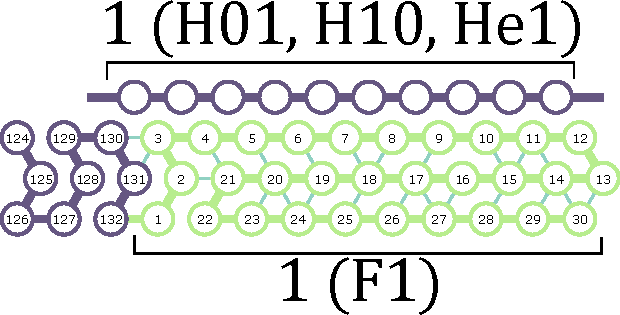
\includegraphics[width=0.6\linewidth]{fig/svg/F1_1.pdf}
 \caption{フォーマットモジュールのブリックは全部で4種類存在する。上二つの\texttt{Fnt}と\texttt{Fnb}はジグでのみ現れ、下二つの\texttt{F0}と\texttt{F1}はザグにのみ現れる。}
 \label{fig:formatters}
\end{figure}


\begin{figure}[p]
\centering
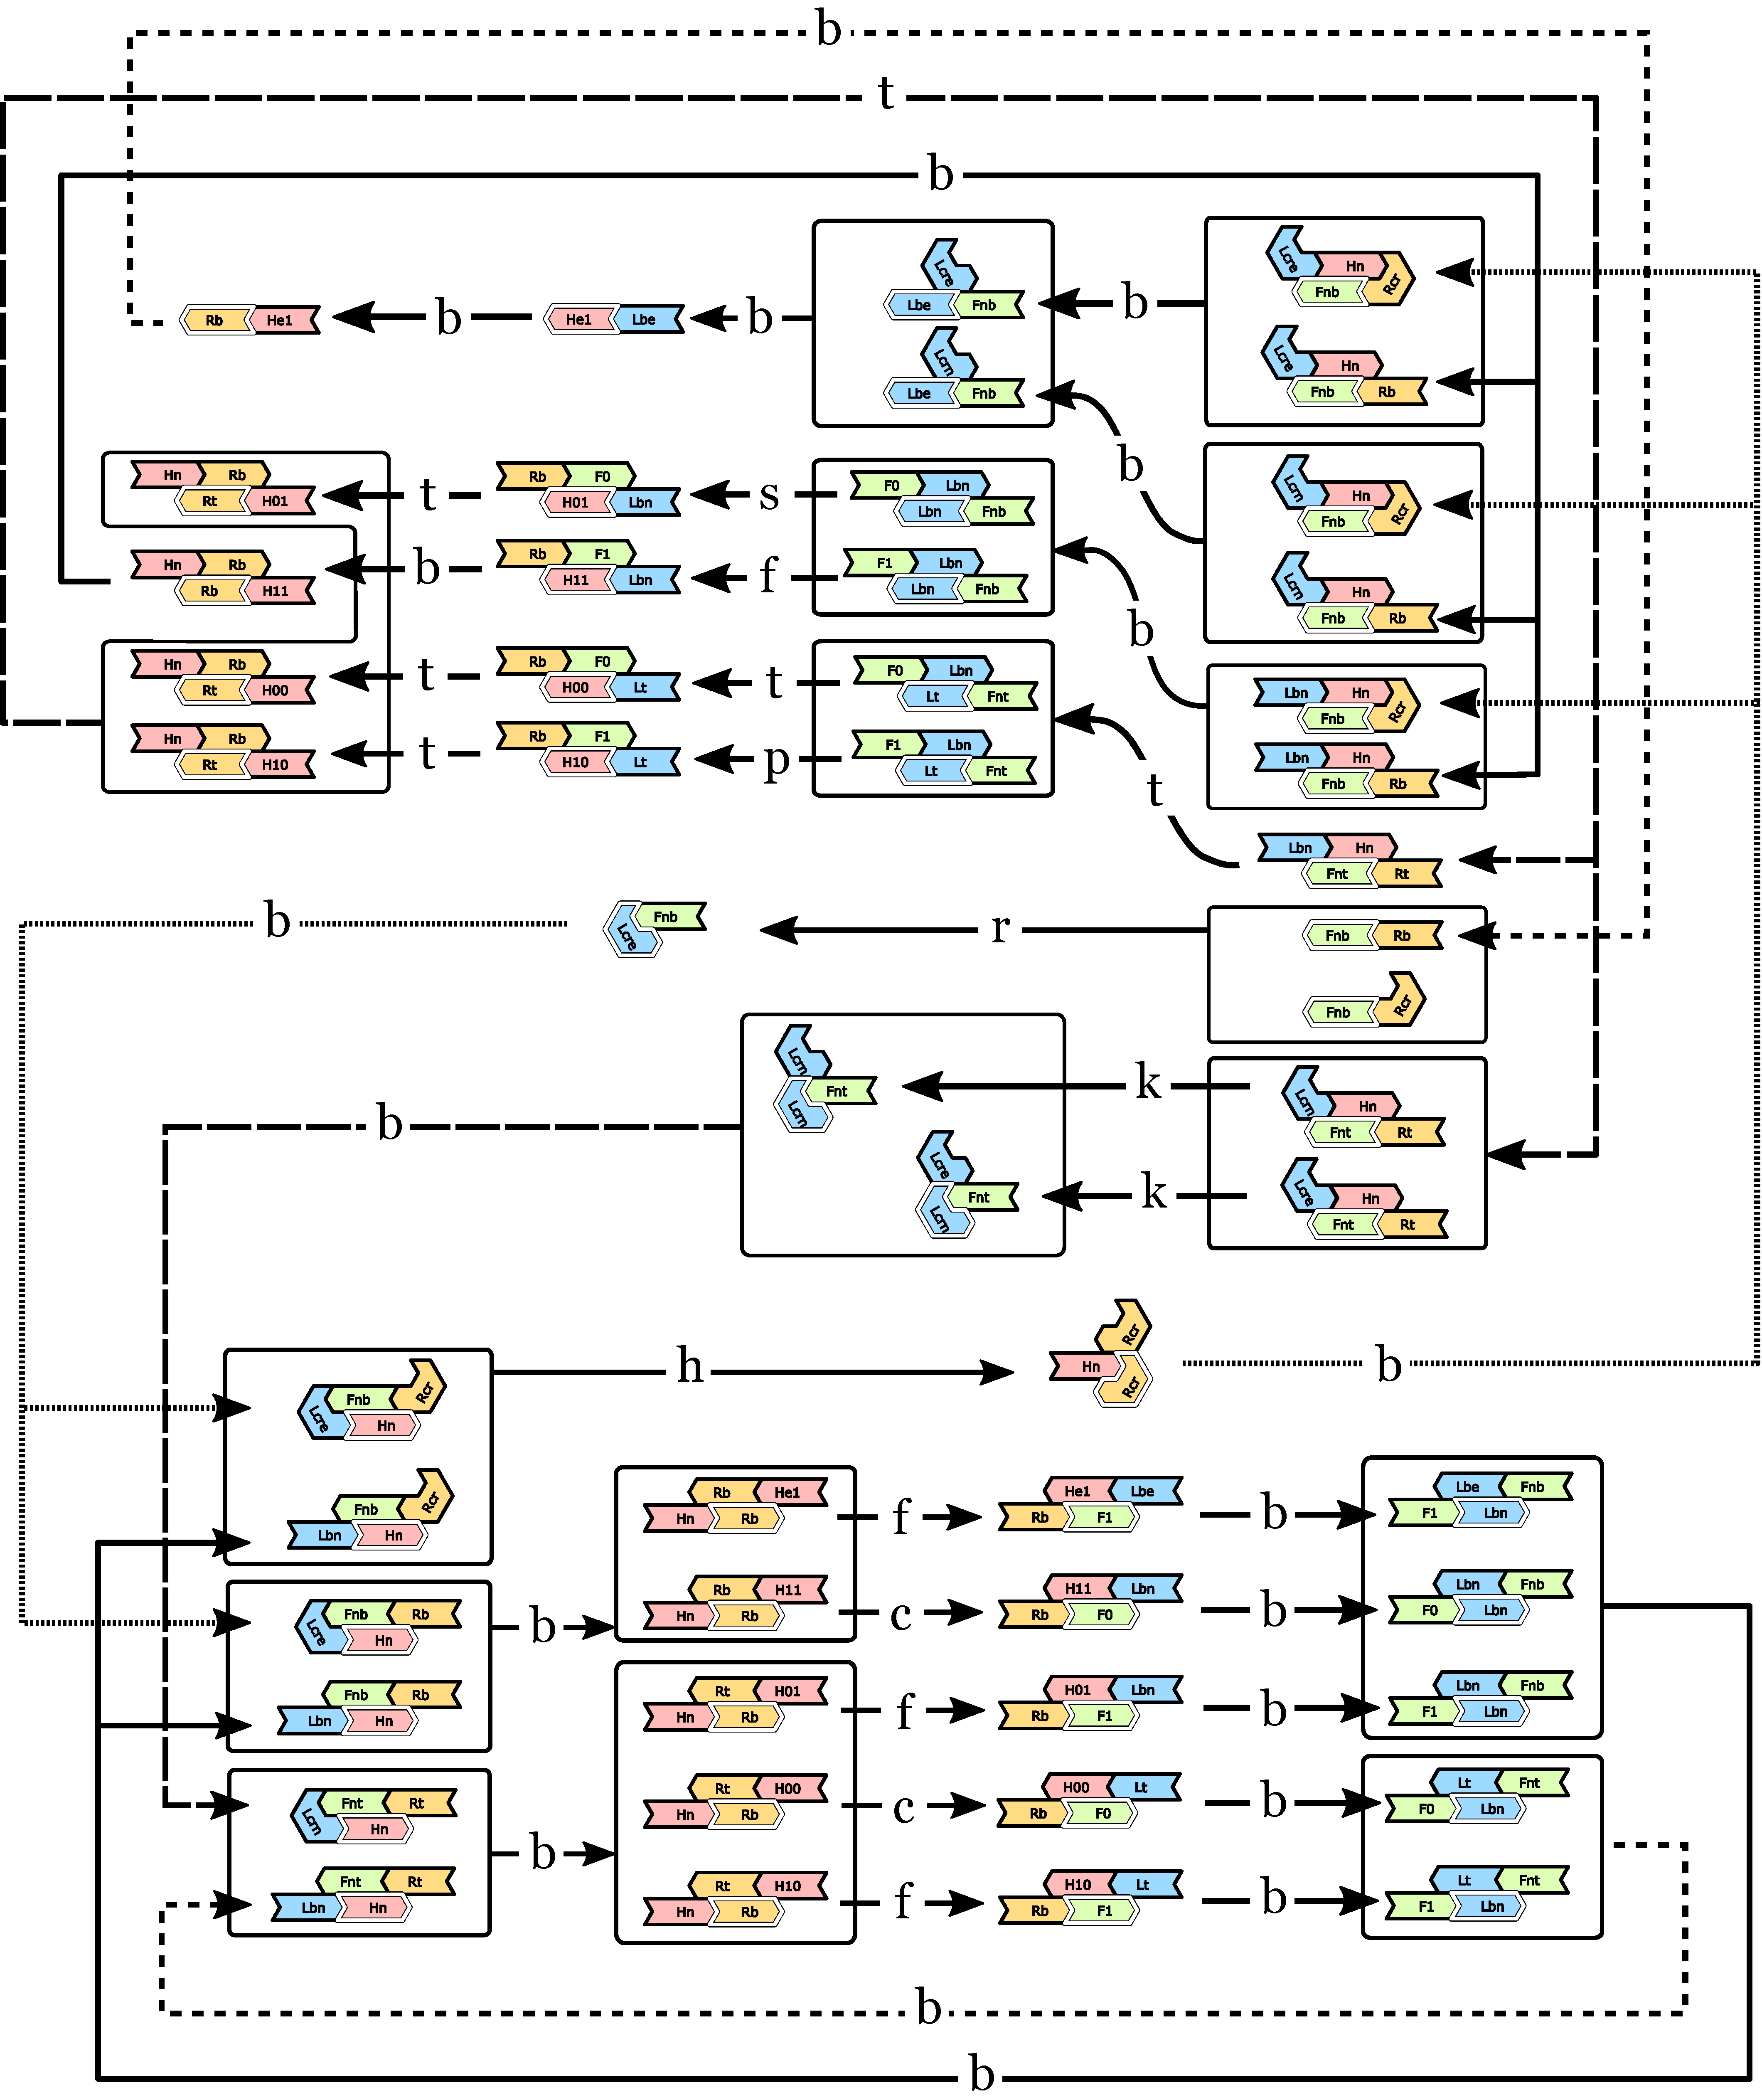
\includegraphics[width=0.95\textwidth]{fig/svg/inf-ai_c_2.pdf}
\vspace*{4mm}

\scalebox{0.68}{
\begin{tikzpicture}
	\node[anchor=north, inner sep=0] (tg) at (0,0) {
 		   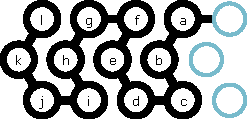
\includegraphics[width=0.2\textwidth]{fig/svg/tglider.pdf}
	};
	\node[anchor=north, inner sep=0] (bg) at (3,0) {
 		   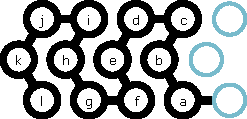
\includegraphics[width=0.2\textwidth]{fig/svg/bglider.pdf}
	};
	\node[anchor=north, inner sep=0] (pl) at (6,0) {
 		   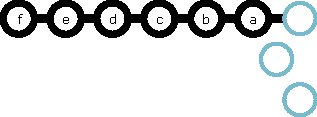
\includegraphics[width=0.2\textwidth]{fig/svg/plane.pdf}
	};
	\node[anchor=north, inner sep=0] (sp) at (9,0) {
 		   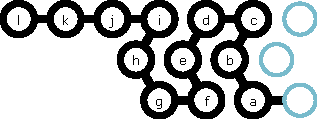
\includegraphics[width=0.2\textwidth]{fig/svg/spiral.pdf}
	};
	
	\node[anchor=north, inner sep=0] (ho) at (-1.5,-3) {
 		   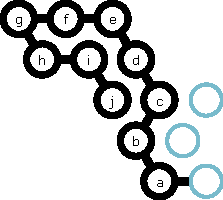
\includegraphics[width=0.2\textwidth]{fig/svg/horn.pdf}
	};
	\node[anchor=north, inner sep=0] (ka) at (1.5,-3) {
 		   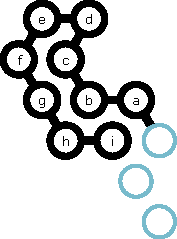
\includegraphics[width=0.15\textwidth]{fig/svg/kar.pdf}
	};
	\node[anchor=north, inner sep=0] (ro) at (4.5,-3) {
 		   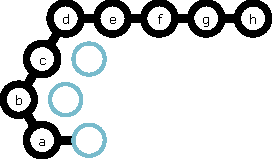
\includegraphics[width=0.2\textwidth]{fig/svg/roof.pdf}
	};
	\node[anchor=north, inner sep=0] (fa) at (7.5,-3) {
 		   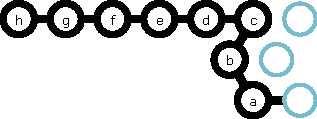
\includegraphics[width=0.2\textwidth]{fig/svg/fault.pdf}
	};
	\node[anchor=north, inner sep=0] (ci) at (10.5,-3) {
 		   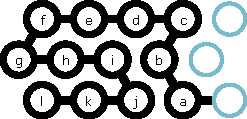
\includegraphics[width=0.2\textwidth]{fig/svg/cliff.pdf}
	};
	
	\node[below, shift=(-90:0.8)] at (tg) {t};
	\node[below, shift=(-90:0.8)] at (bg) {b};
	\node[below, shift=(-90:0.8)] at (pl) {p};
	\node[below, shift=(-90:0.8)] at (sp) {s};

	\node[below, shift=(-90:1)] at (ho) {h};
	\node[below, shift=(-90:1)] at (ka) {k};
	\node[below, shift=(-90:0.8)] at (ro) {r};
	\node[below, shift=(-90:0.8)] at (fa) {f};
	\node[below, shift=(-90:0.8)] at (ci) {c};
\end{tikzpicture}
}
\caption{無限バイナリカウンタのブリックオートマトン}
\label{fig:brickautomaton}
\end{figure}

%%%%%%%
%%%%%%%

\subsection{挙動の概要}
Geary らは有限バイナリカウンタを oritatami system に実装することに成功している\cite{GeMeScSe2019}。
今回実装した無限バイナリカウンタもオーバーフローしていない部分のカウントアップについては、この有限カウンタと同じような振る舞いをする。
具体的には、いずれの\textit{transcript}もジグザク構造をとるように折りたたまれ、そのジグザグは段重ねになり一定方向(この章で用いる図では下方向)に伸びていく。
またジグザク構造のうち、ジグ(右から左への伸長)では現在のカウントが1つカウントアップされ、次のザグ(左から右への伸長)ではジグでカウントアップされた値をフォーマットし、次のジグのためにその値を下方向へコピーする。
無限カウンタと有限カウンタで異なるのはオーバーフローに遭遇した時の挙動である。
無限カウンタはビット幅を1つ拡張することによってカウントアップを続行する。

実装した無限カウンタの\textit{transcript}は同じ塩基配列を周期的に繰り返す。
その1周期分の塩基配列は、\texttt{1}-\texttt{2}-\texttt{3}- $\cdots$ -\texttt{132}であり、更にこれは「モジュール」と呼ばれる以下のような4つの部分配列に分けられる。

\begin{itemize}
\item \texttt{1}--\texttt{30}: 「フォーマットモジュール」もしくは「F」と呼ぶ
\item \texttt{31}--\texttt{66}: 「左ターンモジュール」もしくは「L」と呼ぶ
\item \texttt{67}--\texttt{96}: 「半加算器モジュール」もしくは「H」と呼ぶ
\item \texttt{97}--\texttt{132}: 「右ターンモジュール」もしくは「R」と呼ぶ
\end{itemize}

無限カウンタの\textit{transcript}は、この4つのモジュールを用いて$(FLHR)^*$と表すことができる。
また、これらのモジュールは図中ではそれぞれ緑、青、赤、黄色に色分けする。
モジュールはその周囲の環境ごとにそれぞれ特定の平面構造に折りたたまれるように設計されていて、この平面構造のことを「ブリック」と呼ぶ。すなわち、このブリックを「出力」とみなすと、周囲の環境は「入力」であり、oritatami system がモジュールをブリックに折りたたむ過程は情報の「処理」となる。また、出力として扱われたブリックは、別のモジュールにとっての周囲の環境の一部となることによって、情報が伝搬して行く。

例えばフォーマットモジュールについて、そのブリックを見てみる。
フォーマットモジュールは図~\ref{fig:formatters}で示される4種類の環境に遭遇し、それぞれの環境で異なるブリックに折りたたまれる。
これにおいてモジュールがそれぞれのブリックに折りたたまれるのは、式~\eqref{eq:OS_SF}に従って\textit{transcript}内の特定の塩基同士が結合するように設計しているためである。

無限カウンタを実装したsystemは、各モジュールにおいて想定された環境にしか遭遇しないことが図~\ref{fig:brickautomaton}の「ブリックオートマトン」によって保証されている。
この図では頂点して環境とブリックのペアが、頂点間の遷移としてブリックの前半部分が示されていて、さらにこのブリックオートマトンは閉じている。
そのため環境とブリックのペアのすべてについて、各環境でモジュールが正常に目的のブリックに折りたたまれることを確認するだけで、このブリックオートマトンによってsystemが正しく動作していることを保証できる。
動作確認は専用に開発したシミュレータを用いて行われ、その結果は\href{https://komaruyama.github.io/oritatami-infinit-counter/}{\texttt{https://komaruyama.github.io/oritatami-infinit-counter/}}に掲載されている。


\subsection{ブリック単位での動作説明}


\section{$| \Sigma | = 1$における非チューリング完全性について}

\section{まとめ}

\section{謝辞}

\bibliographystyle{plain}
\bibliography{master2020}

\end{document}
